%%%%%%%%%%%%%%%%%%%%%%%%%%%%%%%
\section{Traffic Trends: Content Server Diversity}\label{sec:traffic-diversity}
%%%%%%%%%%%%%%%%%%%%%%%%%%%%%%%

So far we have highlighted that the Web and P2P protocols are responsible for a
major share of the Internet traffic. However, we have not yet explored if all
content is equally popular or if a few content providers dominate. This is the
goal of this section.

Our evaluation methodology relies on packet level traces from a large European
ISP. We analyze them towards identifying CDI infrastructures and their behavior
as seen by an ISP. Here, we find that CDIs rely on the domain Name System (DNS)
for their operation. Thus, we focus our analysis on the DNS infrastructure in
order to find the server deployment, mapping and operational behavior of CDIs.
Based on these observations, we develop classification methods to detect CDI
infrastructures and perform a first potential analysis on the impact of CDI
operation when basic ISP knowledge is available.

\subsection{Residential ISP Traces}\label{sec:traces} We base our study on
three sets of anonymized packet-level observations of residential DSL
connections collected at aggregation points within a large European ISP.  Our
monitor, using Endace monitoring cards, allows us to observe the traffic of
more than 20,000~DSL lines to the Internet.  The data anonymization,
classification, as well as application protocol specific header extraction and
anonymization is performed immediately on the secured measurement
infrastructure using the Bro NIDS~\cite{bro-paper} with dynamic protocol
detection (DPD)~\cite {dreger06dpd}.

We use an anonymized 24\,h packet trace collected in March 2010 (\martrace) for
detailed analysis of the protocol behavior. For studying longer term trends, we
used Bro's online analysis capabilities to collect an anonymized protocol
specific trace summary (\httplong) spanning 2 weeks. Additionally, we collected
an anonymized 5\,day DNS trace (\dnslong) in February 2010 to achieve a better
understanding of how hostnames are resolved by different sites. Due to the
amount of traffic at our vantage point and the resource intensive analysis, we
gathered the online trace summaries one at a time. Table \ref{tab:traces}
summarizes the characteristics of the traces, including their start, duration,
size, and protocol volume.  It is not possible to determine the exact
application mix for the protocol specific traces, as we only focus on the
specific protocol.  However, we use full traces to cross check the general
application mix evolution.

\begin{table*}
  \small
    \begin{center}
      \tabcolsep2mm
      \begin{tabular}{l|l|l@{ }l|r|r|r}

      Name      & Type     & \multicolumn{2}{|l|}{Start date} & Dur. & Size        & Application Volume \\
      \hline
      \martrace & packet   & 04 Mar'10    & 2am    & 24~h      & $>$5\,TB    & $>$ 3\,TB HTTP, $>$ 5\, GB DNS \\
      \hline
      \httplong & log file & 09 Sep'09    & 3am    & 14~d      & $>$ 200\,GB & corresponds to $>$ 40\,TB HTTP \\
      \dnslong  & packet   & 24 Feb'10    & 4pm    & 5~d       & $>$25\,GB   &  $>$ 25\,GB DNS \\
      \end{tabular}
    \end{center}
    \vspace*{-1\baselineskip}
    \caption{Summaries of anonymized traces from a European ISP}%
    \label{tab:traces}
\end{table*}

With regards to the application mix, recall Section~\ref{sec:traffic}, Maier et
al.~ \cite{OnDominantCharacteristics2009} find that HTTP, BitTorrent, and
eDonkey each contribute a significant amount of traffic, see Table
\ref{tab:traces}.  In \martrace HTTP alone contributes almost 60\perc of the
overall traffic at our vantage point, BitTorrent and eDonkey contribute more
than 10\perc. Recall that similar protocol distributions have been observed at
different times and at other locations of the same ISP, see
Figure~\ref{fig:related:appmix} summarizes the results. Note that almost all
streaming is done via the Web on top of HTTP.  Therefore, we conclude that
currently HTTP is the dominant service and P2P is still responsible for at
least 15\% of the traffic.

Analyzing \httplong, we find more than 1.2 billion HTTP requests, or 89 million
requests per day on average. This is consistent with 95 million requests in 24
hours in \martrace. The advantage of using click stream data from a large set
of residential users is their completeness. We are, e.g., not biased by the
content offered \first by a web service, \second whether sufficient users
installed measurement tools such as the \url{alexa.com} toolbar, or \third
whether users actually use some kind of Web proxy.

To identify the most popular web services, we focus on the most popular hosts.
As expected, the distribution of host popularity by volume as well as by number
of requests is highly skewed and is consistent with a Zipf-like distribution as
observed in other studies~\cite{OnDominantCharacteristics2009}. The top 10,000
hosts by volume and the top 10,000 hosts by number of requests together result
in roughly 17,500 hosts.  This indicates that on the one hand, some hosts that
are popular by volume may not be popular by number of requests and vice versa.
On the other hand, there are some hosts that are popular according to both
metrics.  The total activity by these hosts accounts for 88.5\perc of the
overall HTTP volume and more than 84\perc of the HTTP requests. Assuming that
the HTTP traffic volume accounts for roughly 60\perc of the total traffic,
similar to the observations made in September 2009~\cite{OnDominantCharacteristics2009,UGCcacheability} 
and in \martrace, more than 50\perc of the trace's total traffic is captured by
these hosts.

\begin{figure}[htbp]
  \centering
  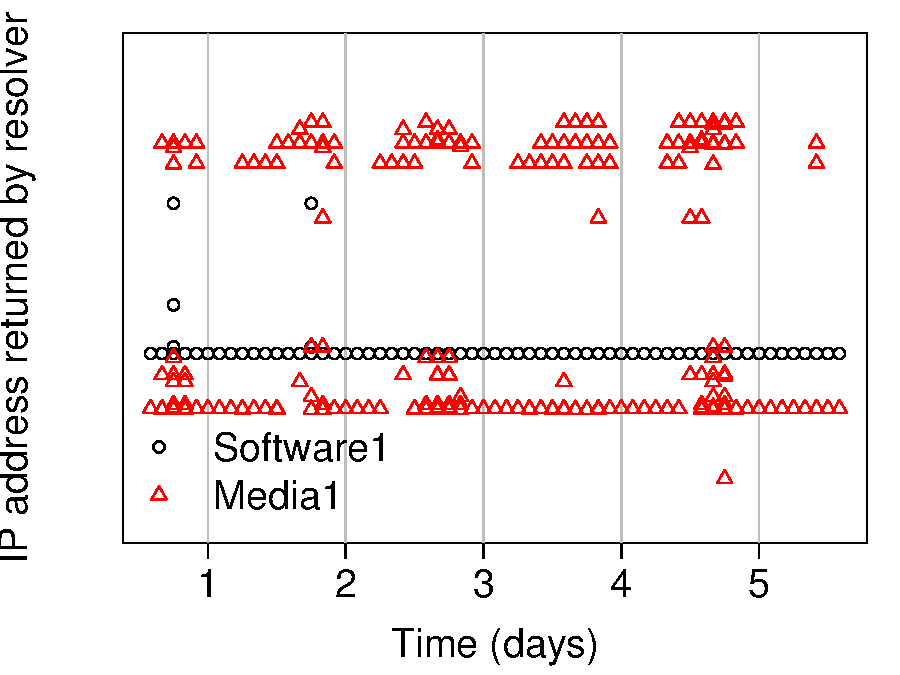
\includegraphics[height=0.7\linewidth]{figures-pdf/dns-diversity}
  \caption{DNS replies for two different sites hosted on a CDI, in two-hour bins.  Reprinted from \cite{PADIS2010}, \copyright ACM, 2010. Included here by permission.}%
  \label{fig:dns_diversity}
\end{figure}


\subsection{Server Diversity and DNS Load Balancing}\label{sec:active_dns_measurement} 

To better understand how HTTP requests are handled and assigned to servers, we
use \dnslong to analyze the 20 most heavily queried DNS names to identify
typical usage patterns. We consider only the most heavily used resolver.
Figure~\ref{fig:dns_diversity} shows two of the typical patterns for two of the
DNS names. It also shows how the resolved IP addresses change (y-axis) across
time (x-axis) for two hostnames; respectively a software site, labeled
Software1, and a media site, labeled Media1. The vertical lines annotate
midnight. If two IP addresses are plotted close to each other, this indicates
that the longest common prefix of the two addresses is close. We note that the
hostname of Software1 is mainly resolved to a single subnet, excepting a few
special cases. However, Media1 is load balanced across approximately 16
different sites. For Media1, there appears to be one main site which is almost
always available, while the remaining 15 are predominantly used during
afternoon and evening peak usage hours.

These results are promising, and show that individual sites do expose a certain
degree of server diversity to their users. While our trace (\httplong) includes
the queried hostnames, it does not include the resolved IP address, as a HTTP
request header contains the hostname but not the IP address of a server. To
verify the above behavior and get an up-to-date view of the DNS replies for the
hostnames of our trace, we used 3 hosts within the ISP to issue DNS queries to
the ISP's DNS resolver for all 17,500 hostnames repeatedly over a fourteen day
measurement period starting on Tue Apr 13th 2010. During these two weeks, we
received more than 16 million replies. Unless otherwise mentioned, we rely on
our active DNS measurements, with augmented statistics concerning volume and
requests from \httplong.

\subsection{Server Location Diversity}\label{sec:server_location_diversity}


Our analysis of hostnames and their assignment to servers in section
\ref{sec:active_dns_measurement} has shown that content can be served by
multiple servers in different locations. In fact, many domains use the service
of a \textit{Content~Delivery~Infrastructure} (CDI), which can be seen during
the DNS resolution progress: The original domain name is mapped to the domain
of a CDI, which then answers requests on behalf of the requested domain name
from one of its caches~\cite{DraftingAkamai:SIGCOMM2006}. Almost all CDIs rely
on a distributed infrastructure to handle the expected load, load spikes, flash
crowds, and special events. Additionally, this introduces needed redundancy and
fail over configurations in their services. Among the most studied CDI' are
Content Distribution Networks (CDNs), such as Akamai~\cite
{ImprovingPerformanceInternet2009, DraftingAkamai:SIGCOMM2006,
MeasuringAndEvaluating2008}, and Content Delivery Platforms (CDPs), such as
Google~\cite{MovingBeyondE2E2009} and their YouTube service~\cite {YouTube}.

\begin{figure}[htbp]
   \center
   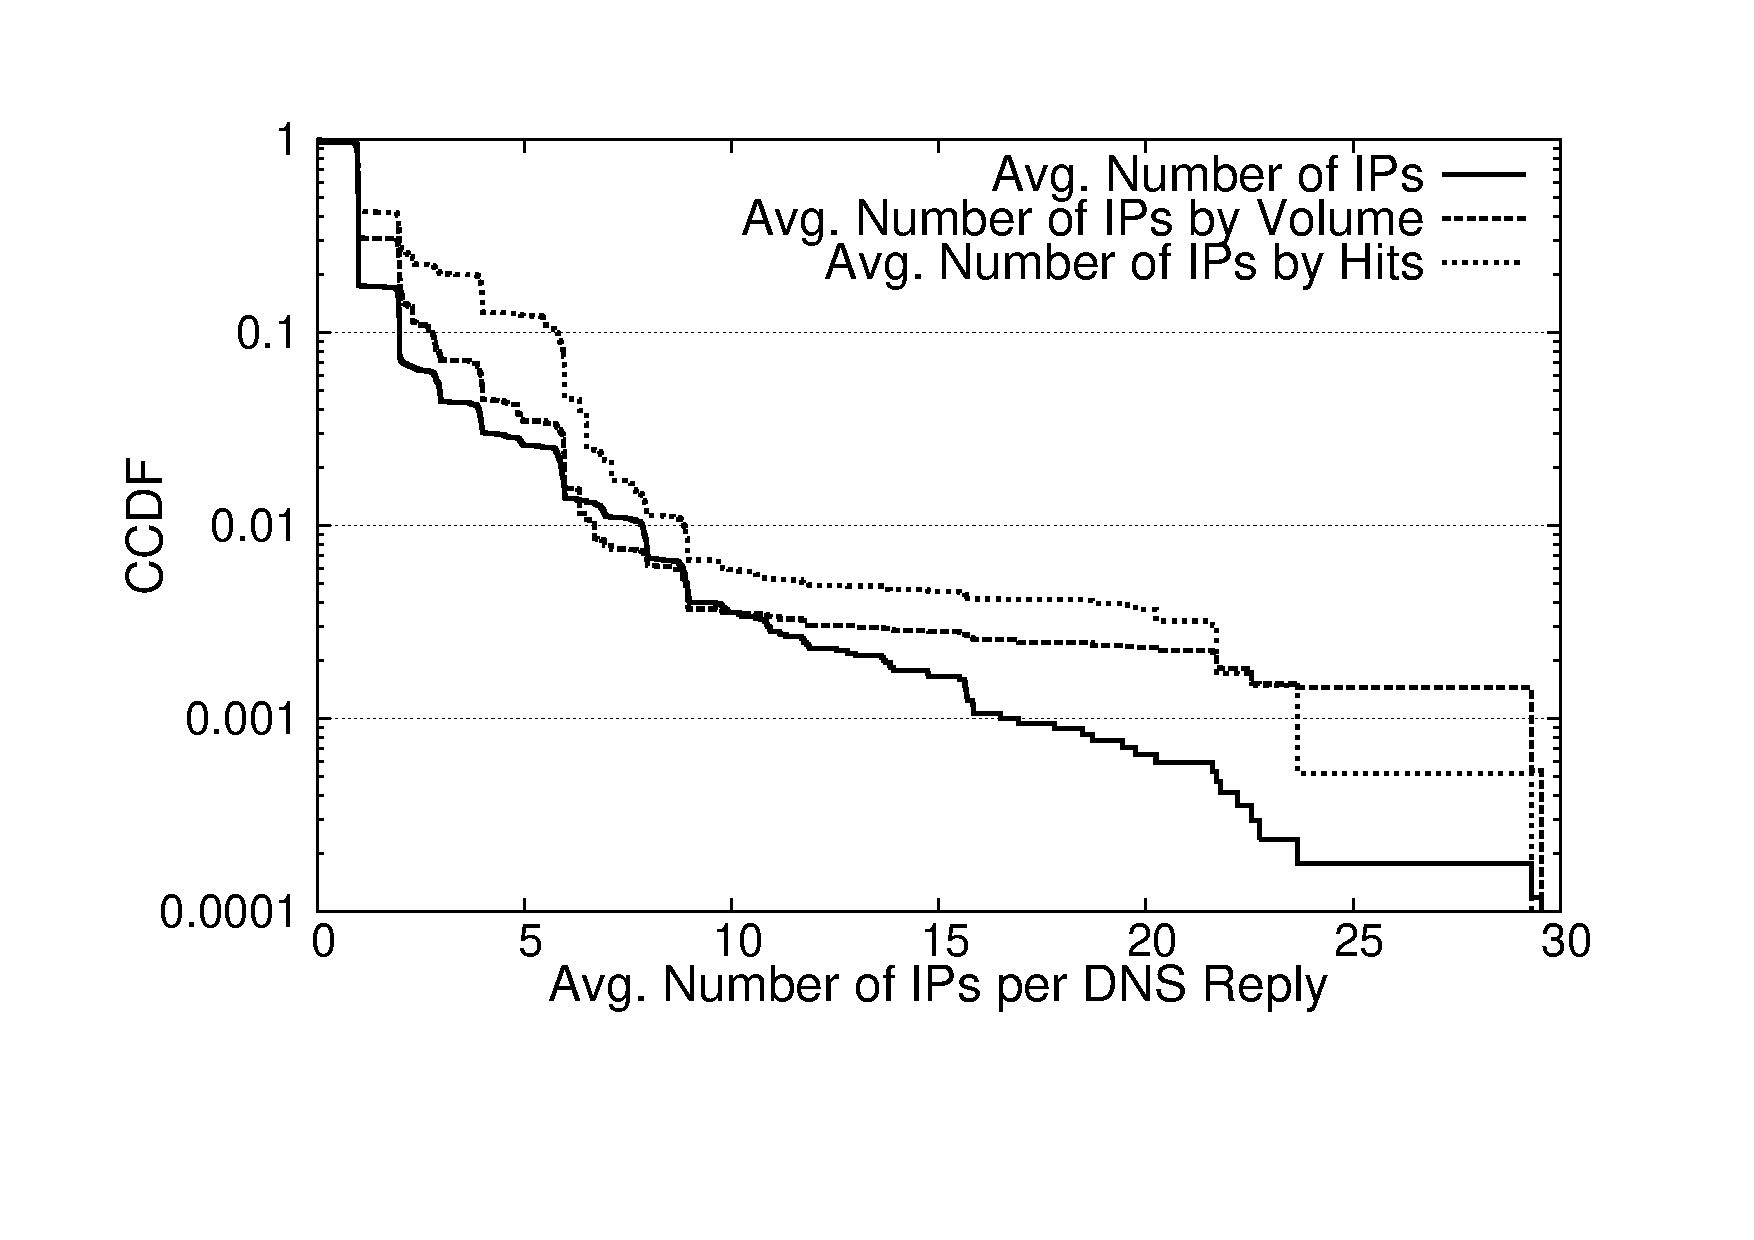
\includegraphics[height=0.7\linewidth]{figures-pdf/avgResponseSize}\\
   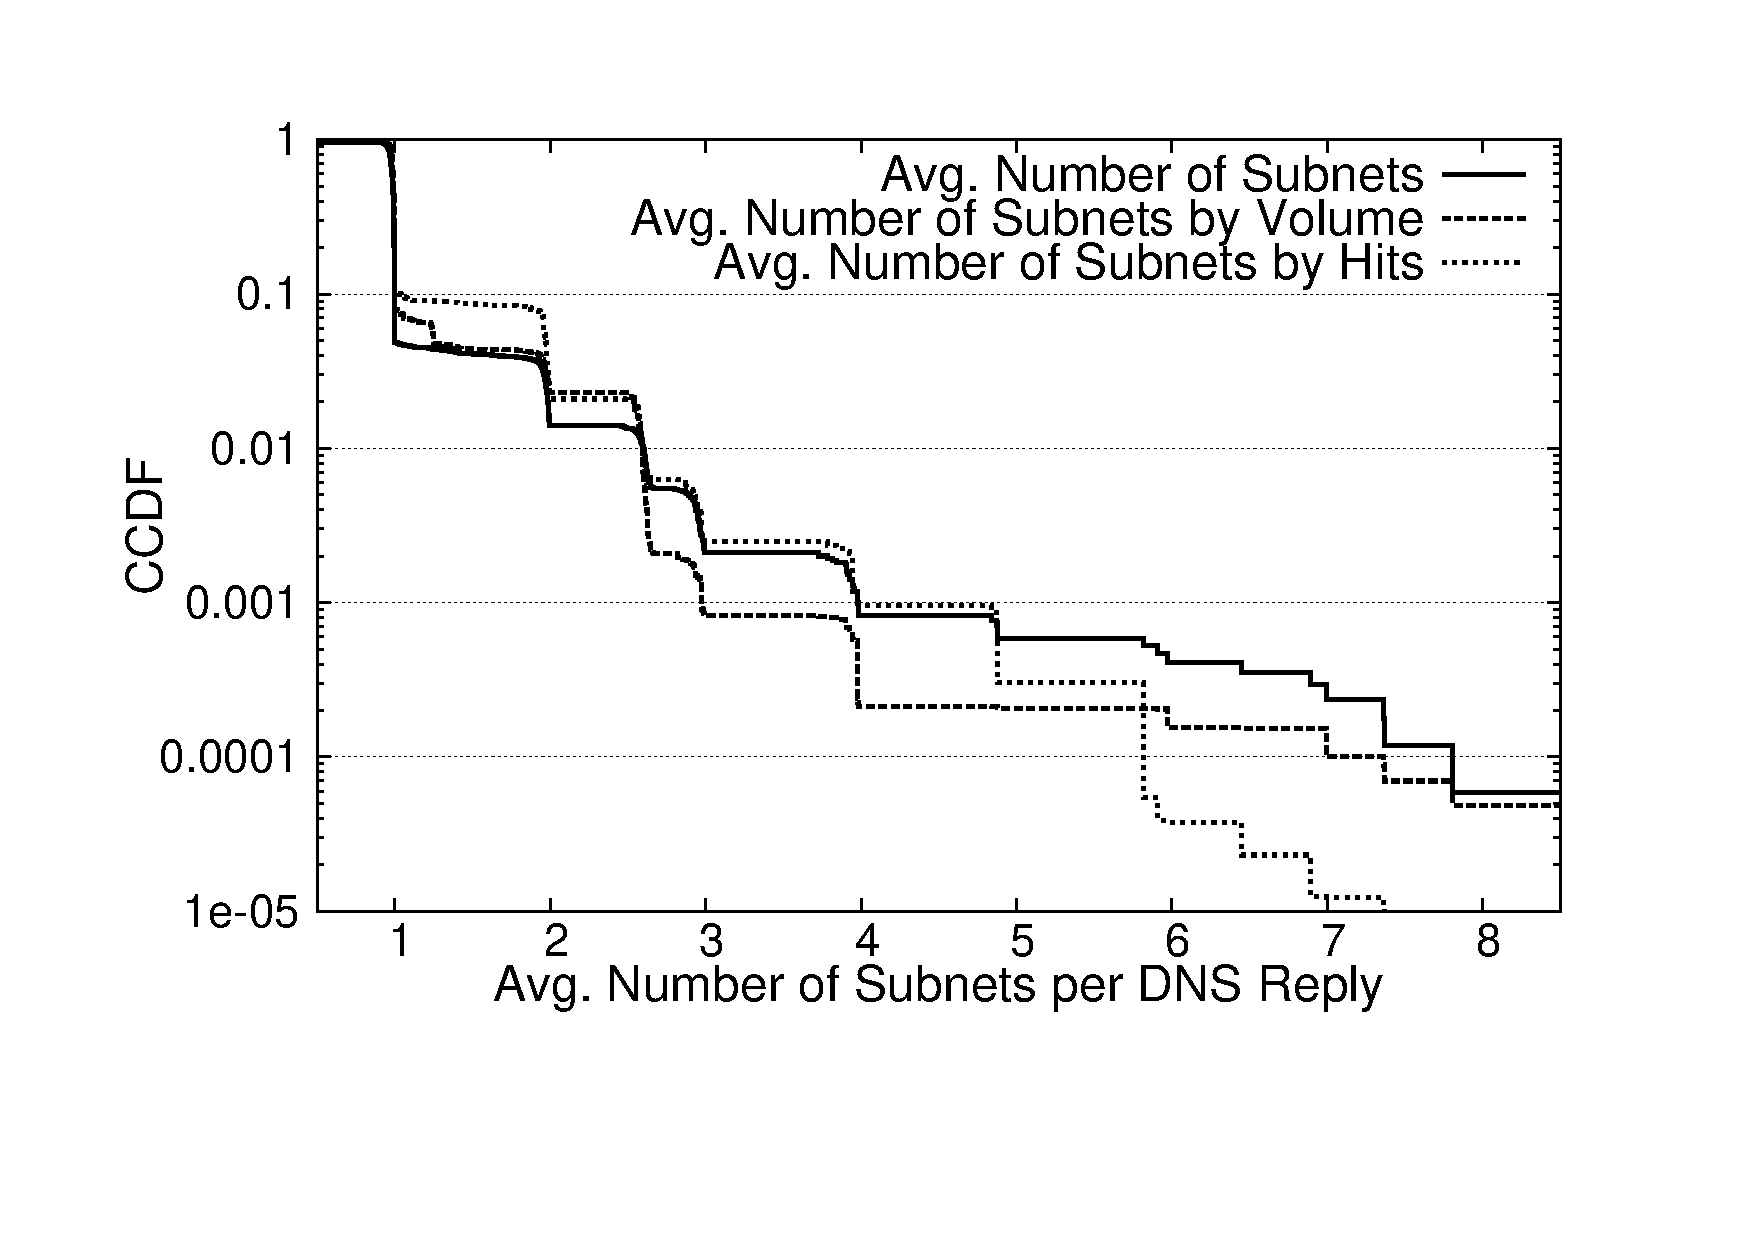
\includegraphics[height=0.7\linewidth]{figures-pdf/avgResponseSubnetSize}

  \caption{CCDF of mean \# of IPs (top) and subnets (bottom) per DNS reply for the ISPs DNS resolver. Reprinted from \cite{PADIS2010}, \copyright ACM, 2010. Included here by permission.}
  \label{fig:CDF-AVG-REPLY-IPs}
\end{figure}

The DNS server can choose to return one or more server IP addresses based on
the domain name in the request and the IP address of the requesting DNS
resolver. For example, it may use a geo-location database~\cite{MaxMind} to
localize the region of the DNS resolver, utilize BGP data to identify the ISP,
create a topology map derived via traceroutes, or any combination of these and
other topological and geographic localization techniques. A DNS server has, in
principle, two methods for load balancing across multiple servers:

\begin{description*}
\item[MultQuery:] Can return multiple IP addresses within a single DNS response
\item[CrossQuery:] Can return different IP addresses for repeated queries and
  thus perform DNS redirection.
\end{description*}

In our active DNS measurements, we found that often a mixture of MultQuery and
CrossQuery is being used in practice. Furthermore, we used the measurement
results to \first map hostnames to sets of IP addresses and \second check the
IP address diversity of these sets for a better understanding of server
diversity and their location. We achieved this by aggregating the returned IP
addresses into subnets based on BGP information obtained from within the
ISP. This allows for detailed information about the different locations within
the ISP, while giving an aggregated view of subnets reachable via peering
links.

Another issue stems from the fact that the IP address returned by the CDI
depends on the IP address of the ISP DNS
resolver~\cite{DNS-IMC-2010,dns-redirection,DraftingAkamai:SIGCOMM2006}. Due to
this, we used the DNS resolver of the ISP of our vantage point as well as
external DNS resolvers (see section \ref{sec:dns_resolvers}). The former
reflects the experience of most of the clients at our vantage point\footnote{We
verify using the traces that more than 95\perc of the clients use the ISP's DNS
resolver as their default one. }. The latter lets us discover additional
diversity as well as understand the preference of the CDI for this specific
ISP.

\begin{figure}[htbp]
  \center
   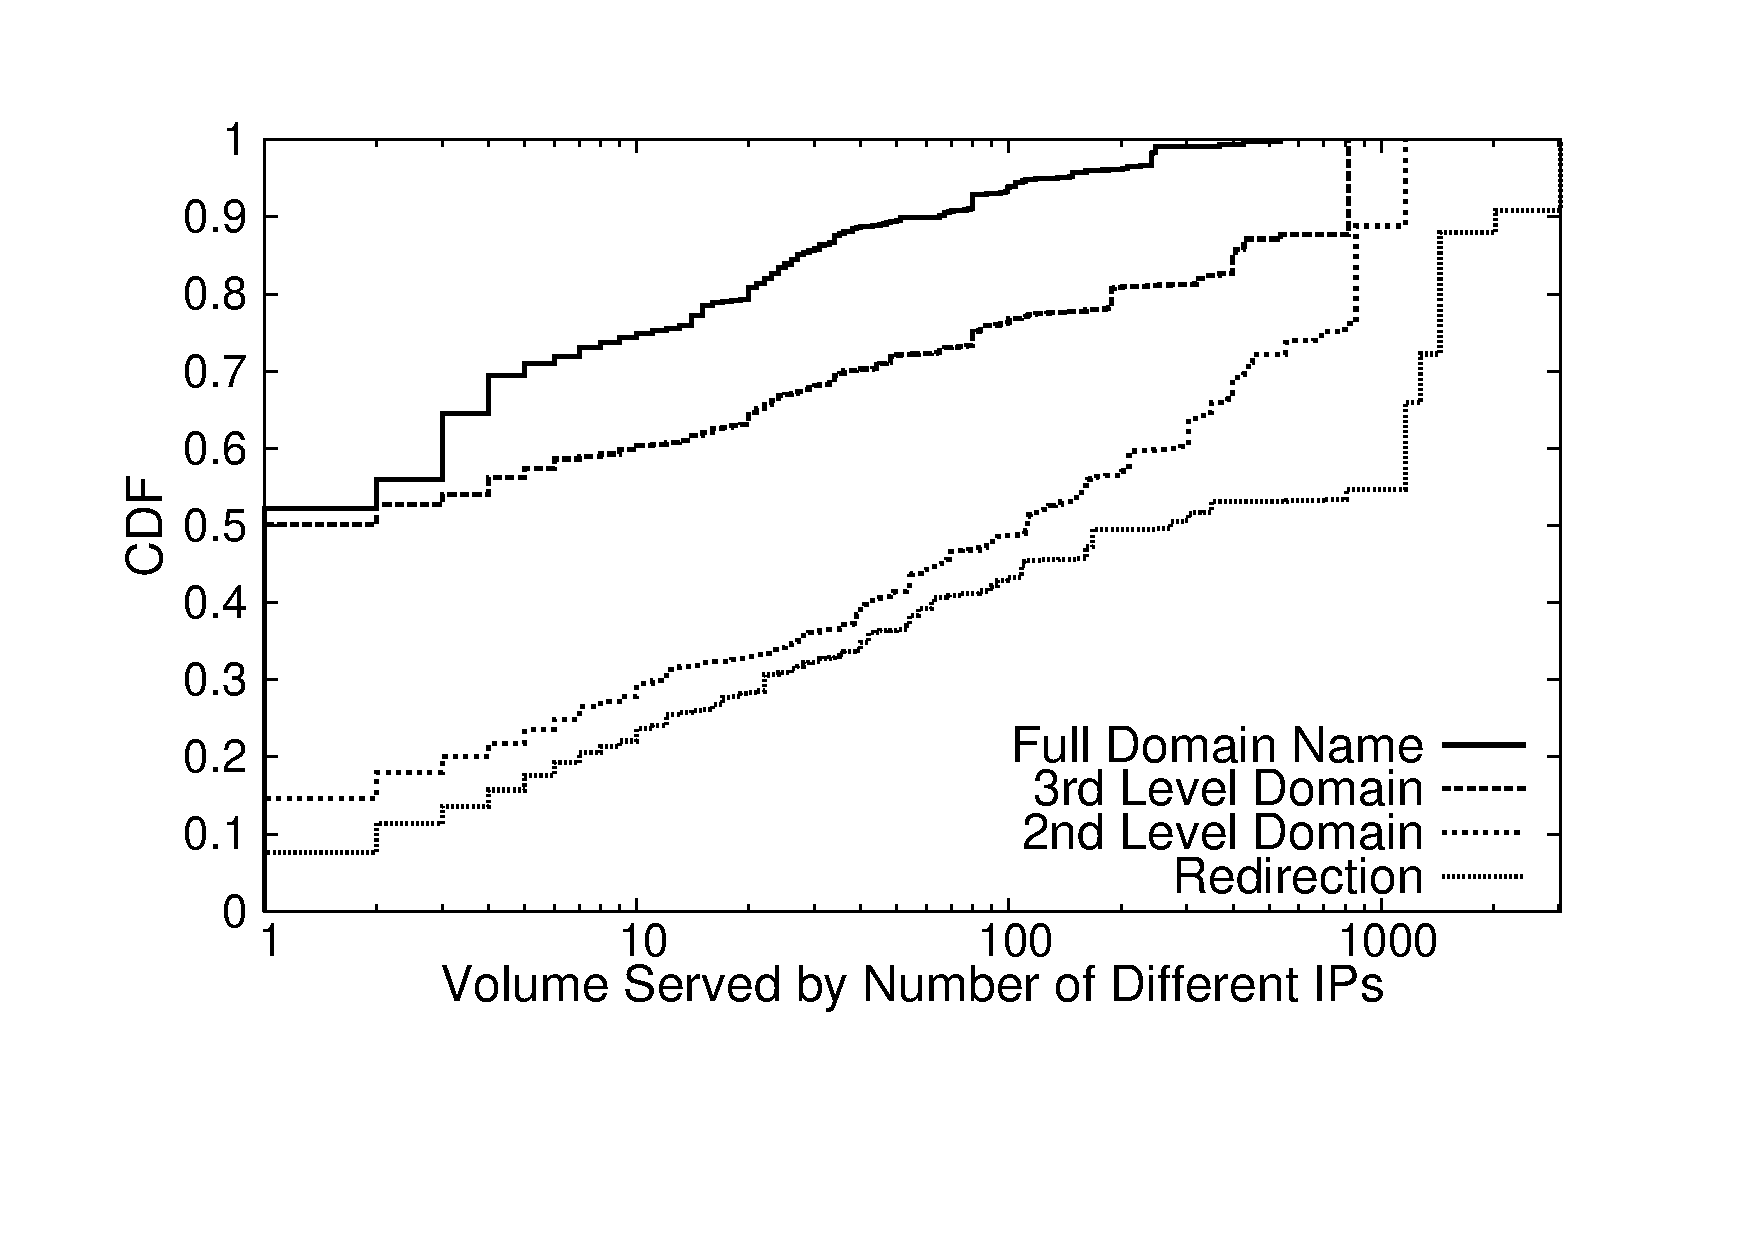
\includegraphics[height=0.7\linewidth]{figures-pdf/14day-returnedIPCDF-bytes}
   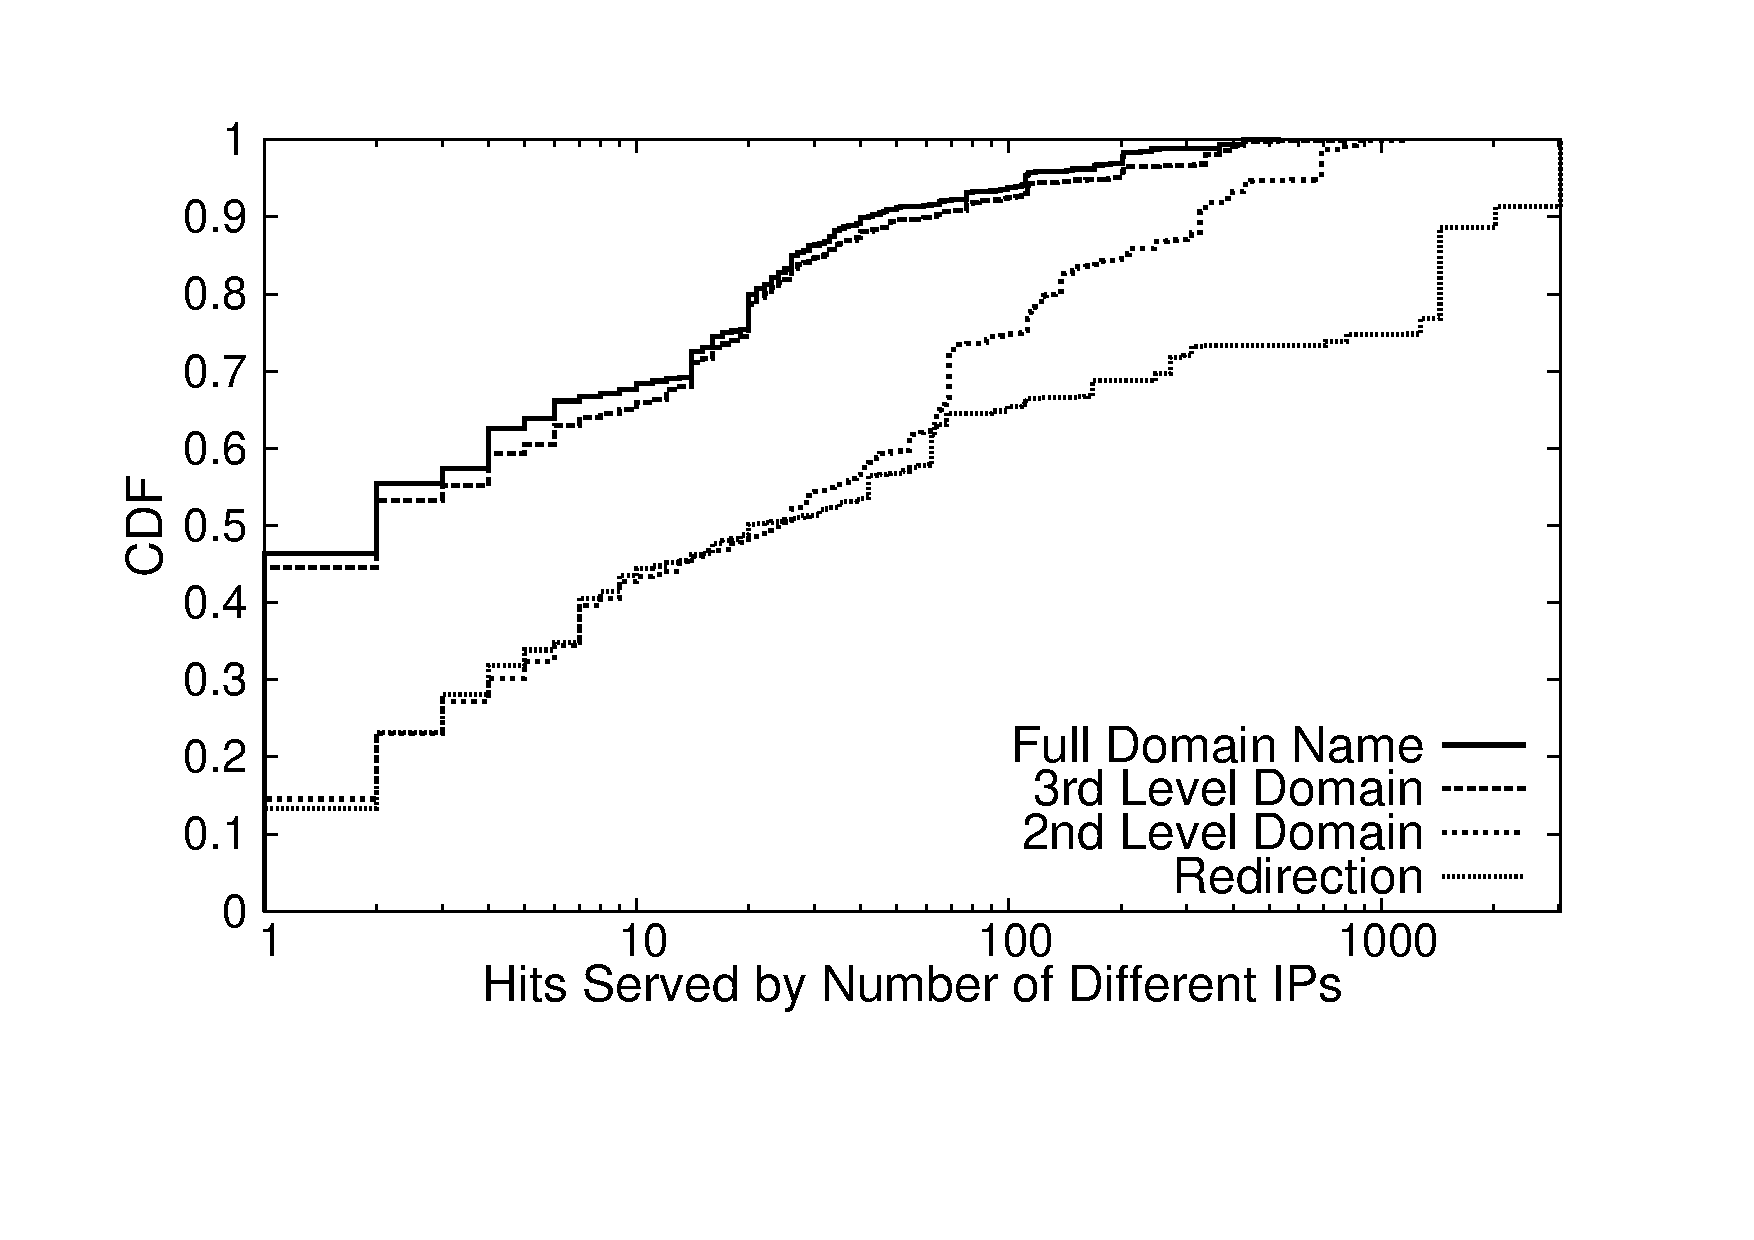
\includegraphics[height=0.7\linewidth]{figures-pdf/14day-returnedIPCDF-hits}
  \caption{CDF of \# of IPs for the ISP DNS resolver normalized by traffic
    volume  (top) and requests (bottom) including aggregation on
    domain levels. (Logarithmic x-axis.) Reprinted from \cite{PADIS2010}, \copyright ACM, 2010. Included here by permission.}
  \label{fig:CDF-IPPAF-IPs}
\end{figure}

\begin{figure}[htbp]
  \center
   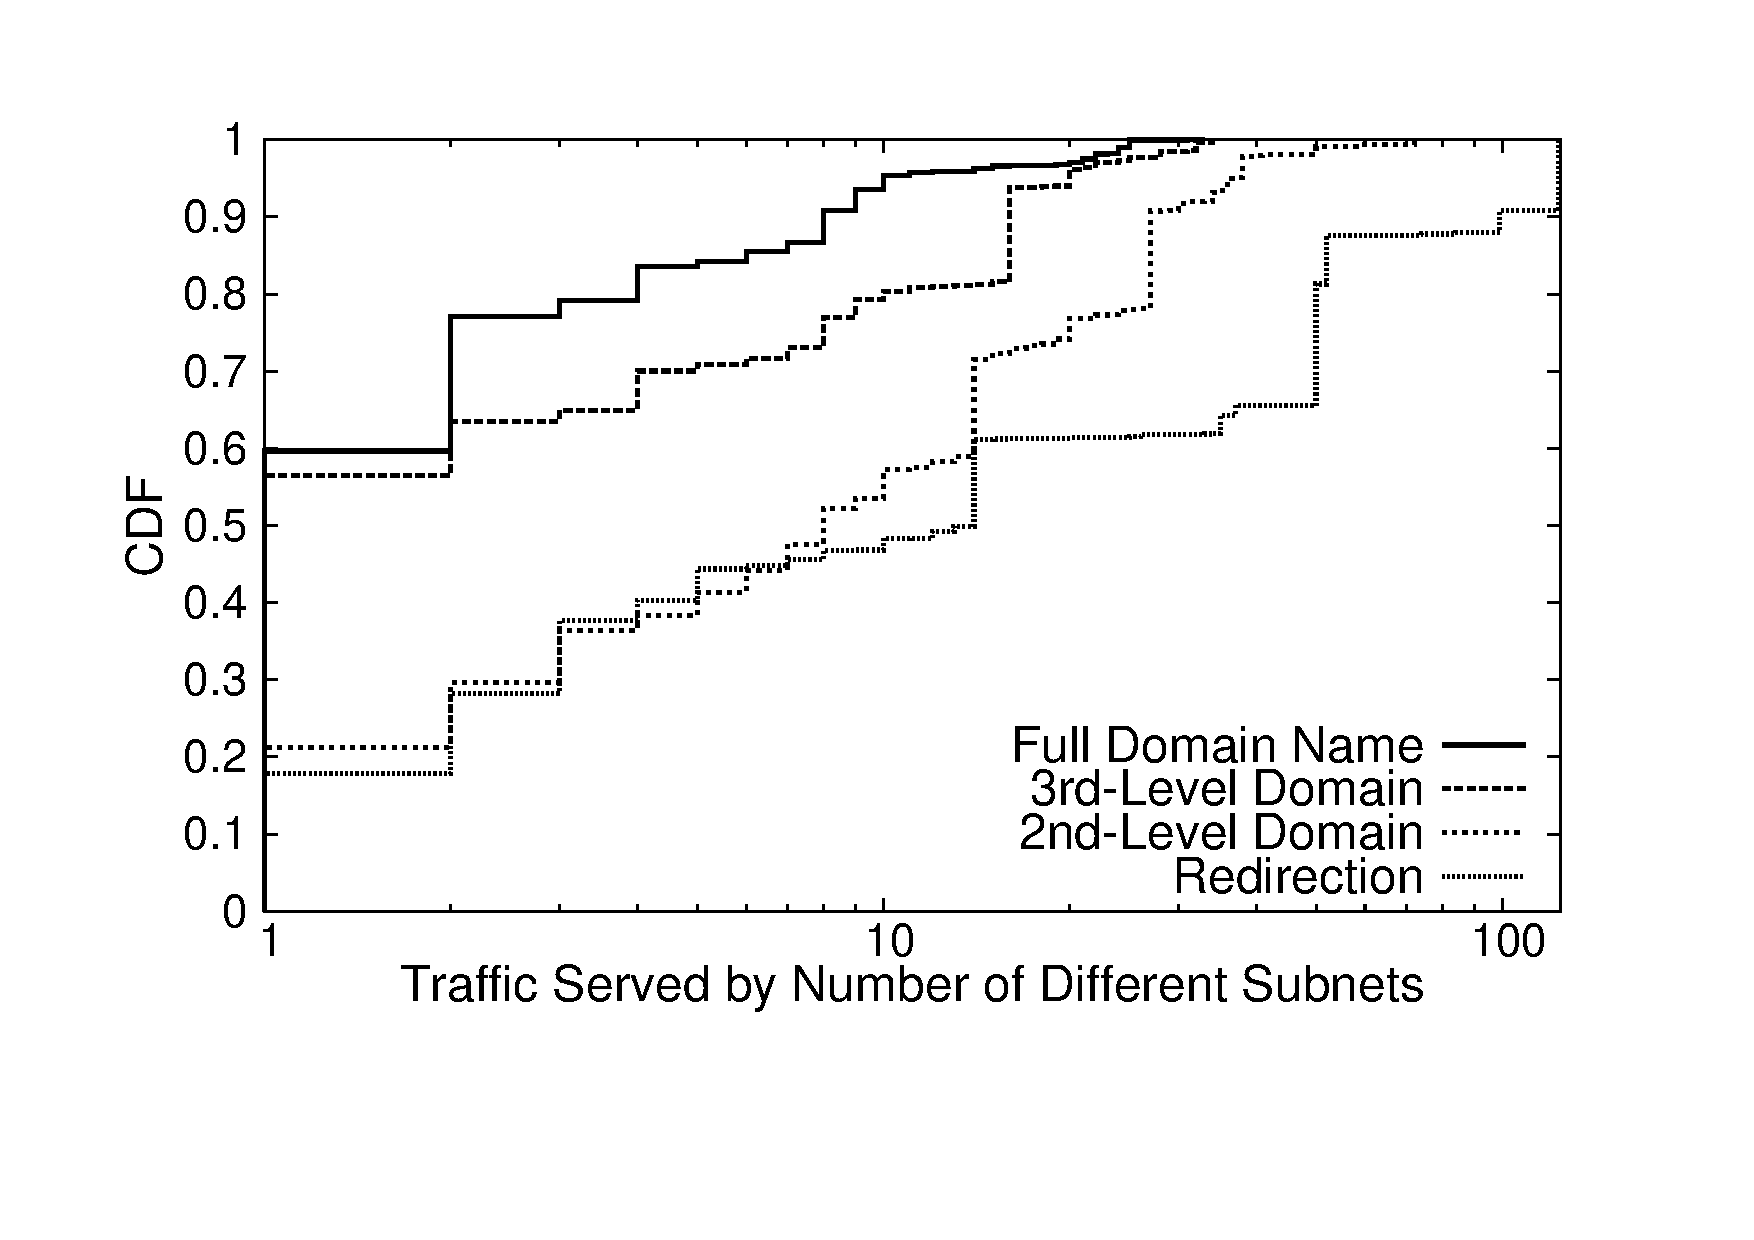
\includegraphics[height=0.7\linewidth]{figures-pdf/SubnetsByBytes}
   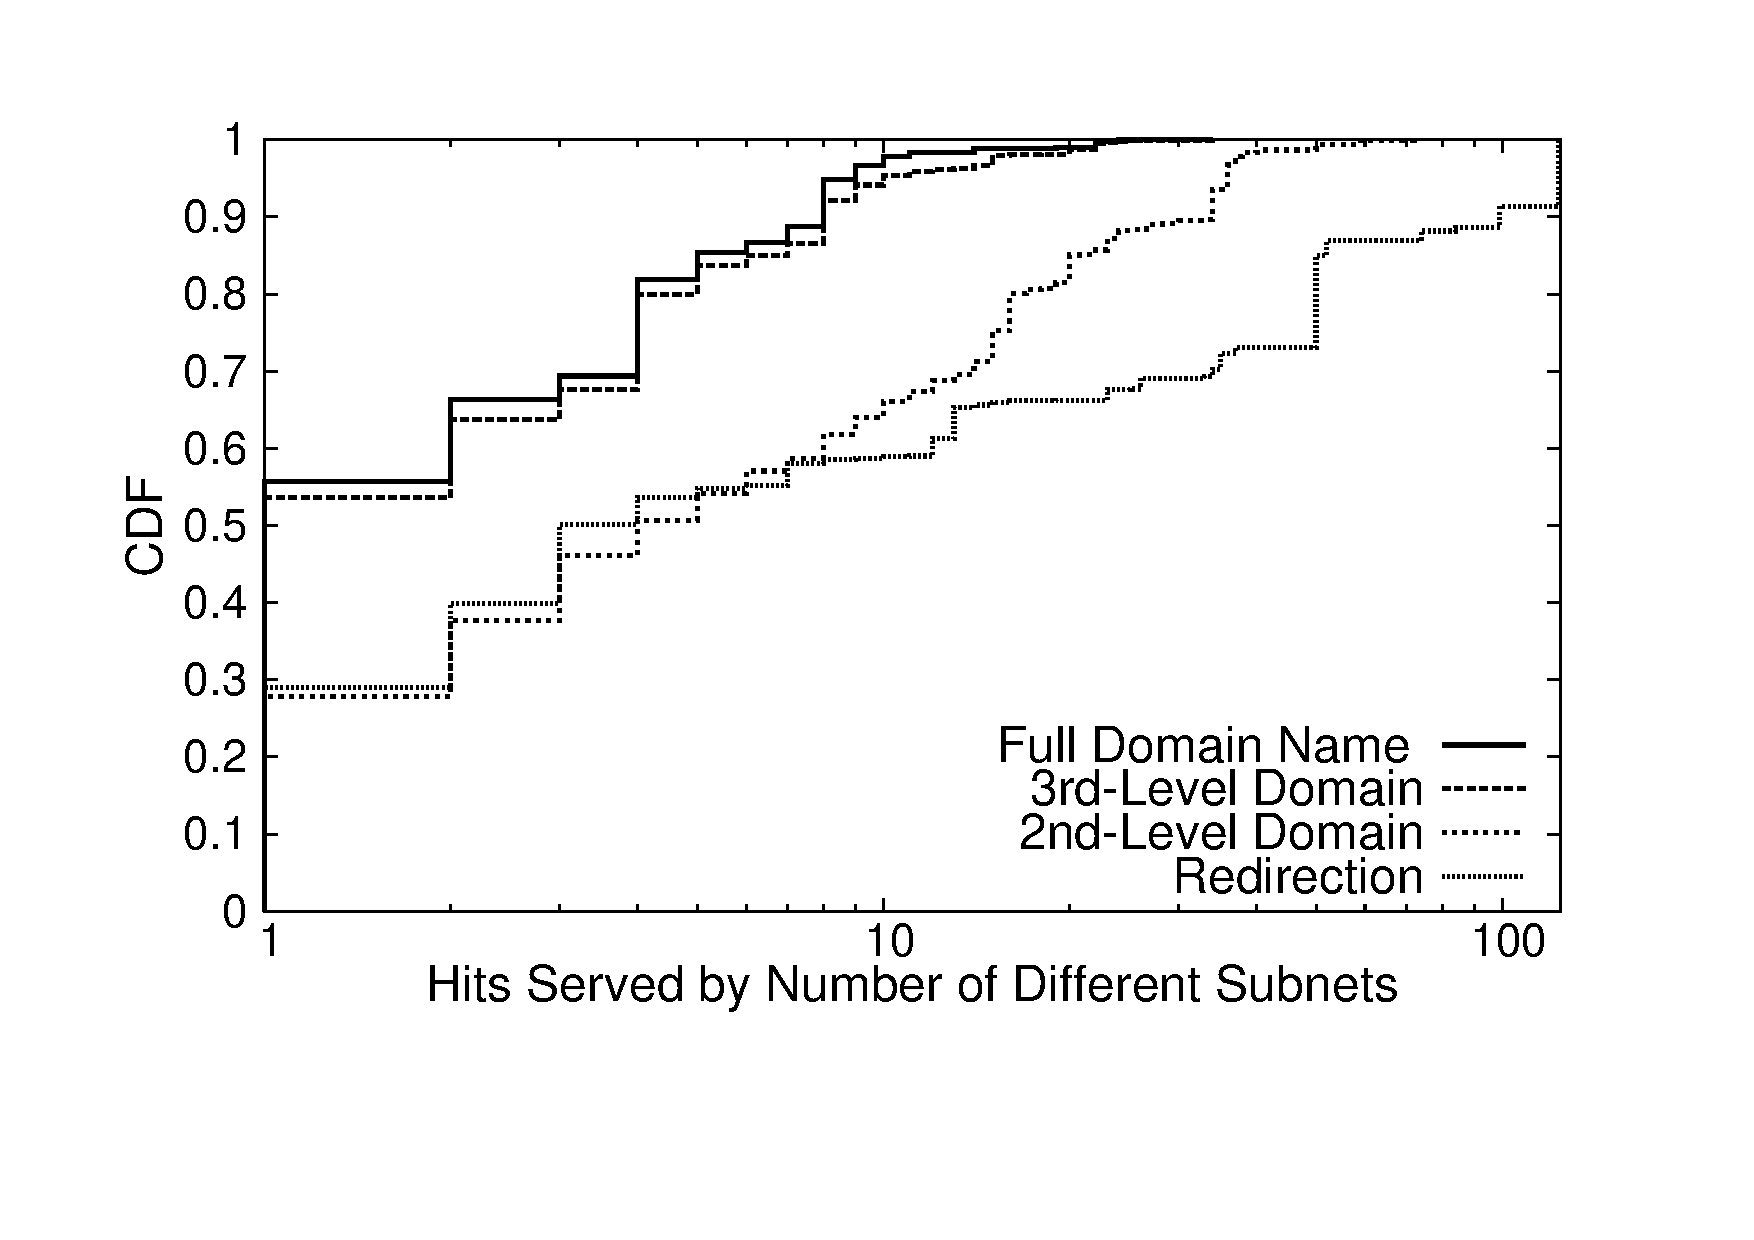
\includegraphics[height=0.7\linewidth]{figures-pdf/SubnetsByHits}
  \caption{CDF of \# of subnets for ISP DNS resolver normalized by traffic
    volume  (top) and by requests (bottom) including aggregation on
    domain levels. (Logarithmic x-axis.) Reprinted from \cite{PADIS2010}, \copyright ACM, 2010. Included here by permission.}
  \label{fig:CDF-IPPAF-Subnets}
\end{figure}

\paragraph{Prevalence of MultQuery.} We start our analysis by checking the
prevalence of the first form of DNS based load balancing, MultQuery. Figure~
\ref{fig:CDF-AVG-REPLY-IPs} shows a CCDF plot of the average number of IP
addresses (top) and subnets (bottom) per DNS reply. In addition, we included
the same data normalized by traffic volume and number of requests.

A first observation is that the number of returned IP addresses per request is
rather small. The median is $1$, the average is $1.3$ and even the $0.9$
percentile is $2$. We note that even when an answer yields multiple IP
addresses, the majority of them are from the same subnet. Therefore, the
diversity decreases even further if we aggregate to subnets. From a network
perspective, this implies that there is not much choice, neither for the ISP
nor for the user, regarding where to download the content from. Both are
limited to the information provided by the DNS server. However, when we
normalize the hosts by their respective popularity, we see a significant
improvement. More than $29$\% of the volume and $19$\% of requests have a
choice among at least $2$ IP addresses.

\paragraph{Prevalence of CrossQuery.} Next, we check how prevalent CrossQuery,
the second form of DNS based load balancing is. Since CrossQuery returns
different IP addresses for repeated queries, its potential contribution to
server diversity can only be studied by aggregating across time. The lines
labeled \texttt{Full Domain Name} in Figures~\ref{fig:CDF-IPPAF-IPs} and~\ref
{fig:CDF-IPPAF-Subnets} capture this case.

We find that more than $50$\perc of the volume or requests can be served by
more than one IP address. Similarly, there is choice between at least two
subnets over $40$\perc of the time across both metrics, see Figure~\ref
{fig:CDF-IPPAF-Subnets}. This indicates that there is significant potential for
the ISP to bias the location preference of the CDI.
\clearpage
\begin{figure}[htbp]
  \center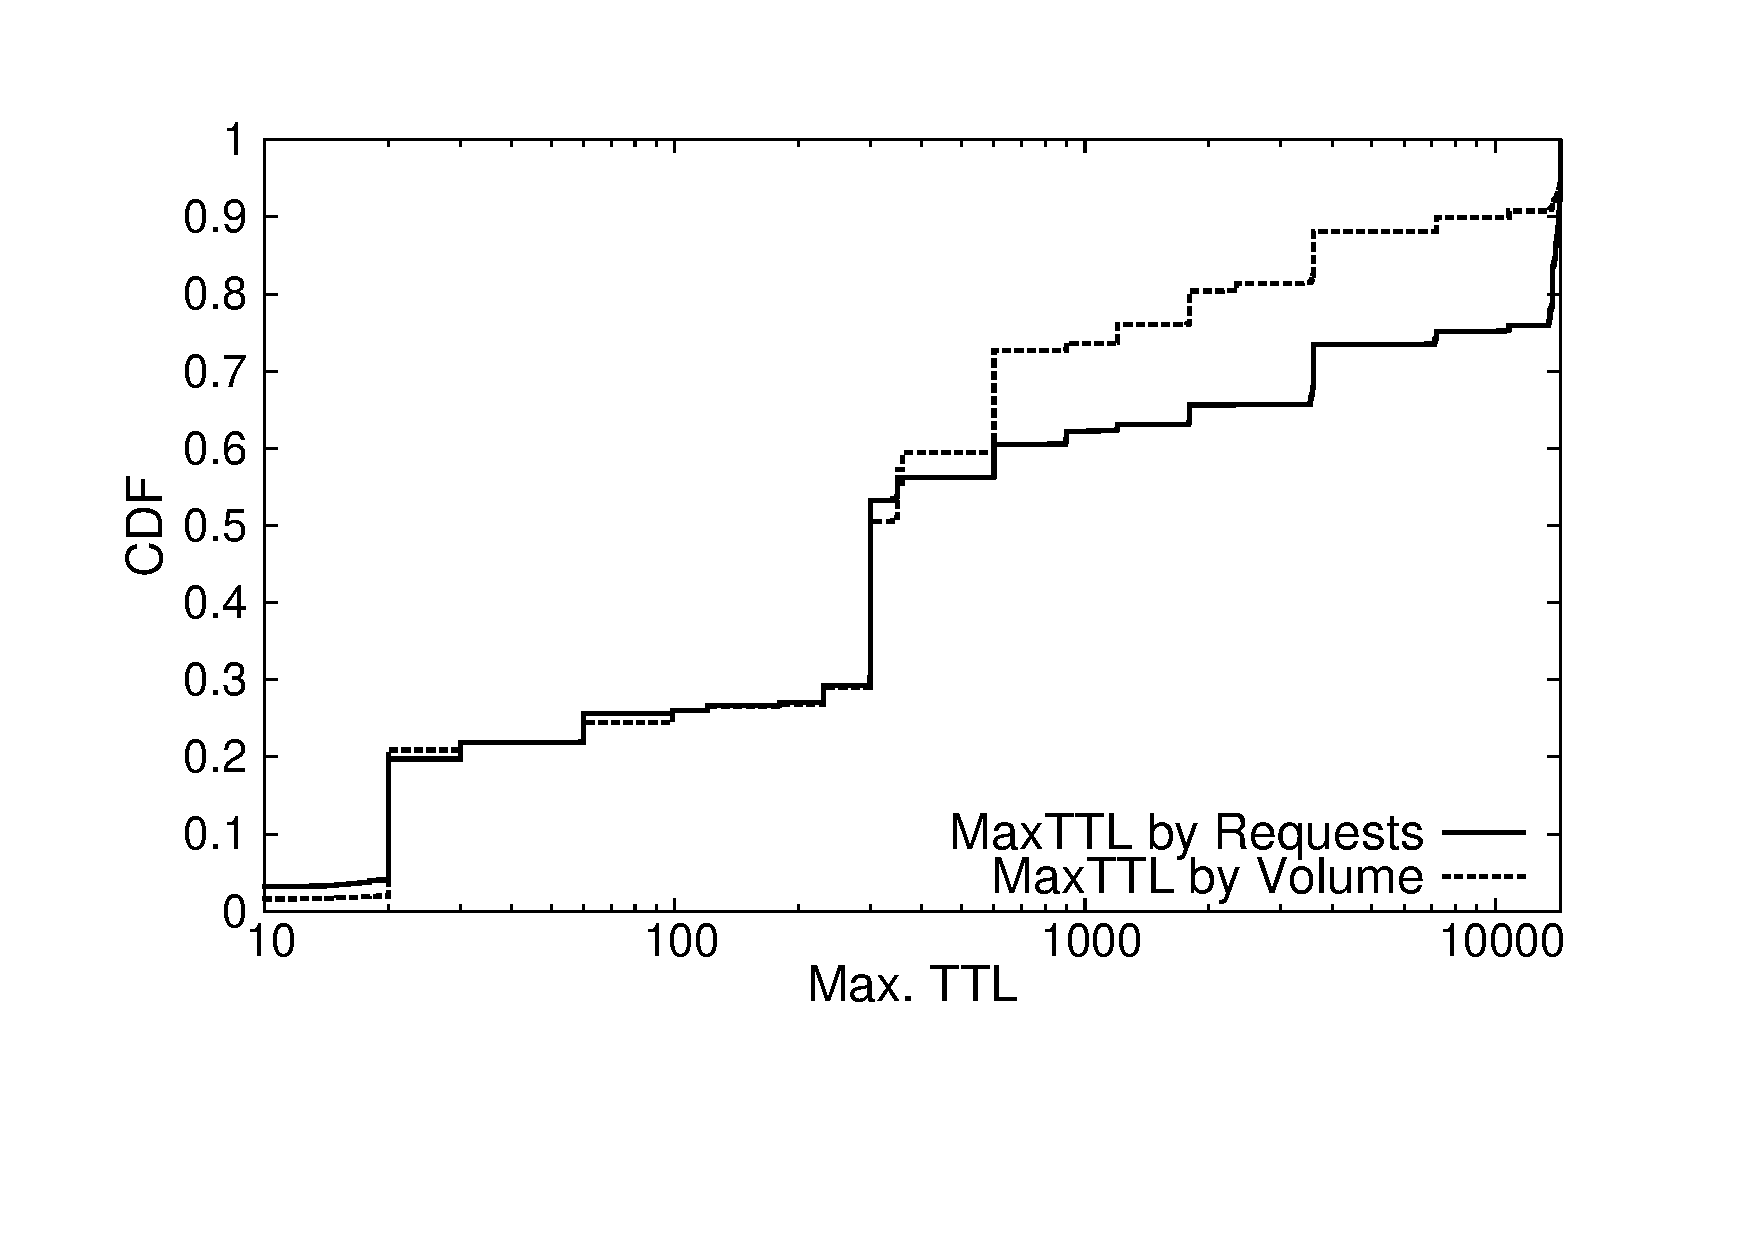
\includegraphics[height=0.7\linewidth]{figures-pdf/maxTTLCDF}
  \caption{CDF of DNS TTL value by traffic volume and by number of requests. Reprinted from \cite{PADIS2010}, \copyright ACM, 2010. Included here by permission.}
  \label{fig:CDF-IPPAF-TTL}
\end{figure}


\paragraph{Subdomain Aggregation.} Since some CDIs only use subdomains as hints
about the context of the requested URLs or the requested services, we
accumulate the answers further regarding the 2nd and 3rd part of the domain
names of the hosts, see Figures~\ref {fig:CDF-IPPAF-IPs}
and~\ref{fig:CDF-IPPAF-Subnets} at the respective data series called
\texttt{3rd Level Domain} and \texttt{2nd Level Domain}. For example, we might
accumulate the IP addresses from DNS replies for \url {dl1.example.org} and
\url{dl2.example.org} for the statistics on the 2nd level domain, but not the
third level domain.

This is a feasible approach, since many hosts respond to all requests that
belong to a subset of the subnets returned when accumulating by the
second-level domain of DNS resolver answer, including recursive requests and
redirections.  This behavior was verified with active measurements
in~\cite{PADIS2010}. We find that at least two major CDIs, a streaming provider
and a One-Click Hoster, serve requested content from servers that match in
their second level domain.

We note that the accumulation by third-level domain, and especially by second
level domain significantly increases the number of observed subnets per request
both normalized by requests as well as by volume.  The number of returned
subnets further increases when accumulating to the second-level domain of DNS
resolver answer. Studying our traces in more detail, we find that this is due
to the substantial traffic volume and number of requests that are served by
CDIs, some of which are highly distributed within ISPs or located in multihomed
datacenters or peer-exchange points.

\paragraph{Infrastructure Redirection Aggregation.}
Taking a closer look at the DNS replies~\cite{ietf-dns}, we find that some CDIs
use CNAME records to map queried hostname to an A record. These A records show
the same pattern as the hostnames in the previous section: the second level
domain is identical. Similar to the previous approach, we can aggregate by
these A records.


Turning our attention to the implications of the proposed aggregation schemes,
we notice the available diversity increases tremendously. More than 50\% of the
hits and 70\% of the bytes can be served by more than $20$ servers.  With
regards to subnets, the diversity decreases slightly. Nevertheless, more than
$5$ subnets are available for 45 \% of the hits and 55\% of the bytes.

If we consider aggregation periods in the order of tens of minutes, the numbers
do not decrease by much.  The reason that most of the diversity is observable
even over these short aggregation time periods, is that the typical TTL, see
Figure~\ref{fig:CDF-IPPAF-TTL}, is rather short with a mean of $2,100$ seconds
and an median of $300$ seconds normalized by volume. When weighted by requests,
the mean/median is $4,100$/$300$ seconds.

\paragraph{Alternative DNS Resolvers.}\label{sec:dns_resolvers}
So far we have only considered the effect of content diversity when the ISP DNS
resolver is used. To understand how much the DNS load balancing deployed by a
CDI is biased by the queried DNS resolver, we repeat the experiment from
Section~\ref{sec:active_dns_measurement} using two other DNS resolvers. In
particular, we pick the next most popular DNS resolvers found in our traces:
GoogleDNS and OpenDNS. Both are third-party resolvers with a global footprint
and utilize DNS anycast.

Comparing the results, we find that we attain more IP address diversity and
subnet diversity when using the ISP DNS resolver. This is mainly due to the
fact that CDIs select the supplied caches based on the source IP address of the
querying DNS resolver. Since the CDIs are no longer able to map the request to
the AS it originates from, but rather to AS the DNS resolver belongs to, the
server selection by the CDI cannot optimize for the location of the DNS client.

A possible solution to the problem is the EDNS-Client-Subnet
extension~\cite{EDNS}, an extension that utilizes the EDNS0 option field that
is used today by DNS Security Extensions (DNSSEC). A recent study~\cite{EDNS:IMC2012} showed that the
user-to-server allocation can be significantly improved as well as the
end-to-end performance for the client. On the other hand, this requires that
all the involved resolvers and authoritative servers in ISPs, CDNs, third
parties that maintain resolvers and authoritative servers, \eg GoogleDNS, OpenDNS, 
have to support EDNS-Client-Subnet extension.



\subsection{Impact on Traffic Localization}\label{sec:dns_localization}

\begin{table}
  \begin{center}
    \tabcolsep2mm{}
    \begin{tabular}{|c||c|c||c|c||c|c|}
      \hline      & \multicolumn{2}{c||}{ISP DNS} & \multicolumn{2}{c||}{OpenDNS} & \multicolumn{2}{c|}{GoogleDNS}\\
      \hline Metric  & observed  & potential & observed & potential   & observed  & potential   \\ \hline
      \hline IPs     & 12.3\perc & 24.2\perc & 5.8\perc  & 16.0\perc  & 6.0\perc  & 9.7\perc    \\
      \hline requests& 14.9\perc & 33.2\perc & 4.7\perc  & 18.8\perc  & 4.8\perc  & 6.4\perc    \\
      \hline volume  & 23.4\perc & 50.0\perc & 12.0\perc & 27.7\perc  & 12.3\perc & 13.4\perc   \\
      \hline
    \end{tabular}
  \end{center}


  \caption{Traffic localization within the network by different DNS resolvers normalized by number of requests and
  traffic volume together with the potentially available fraction of localized traffic.}
  \label{tab:TraceLocallizedTraffic}
\end{table}

Analyzing the three active DNS measurements from the ISP, OpenDNS as well as
Google DNS resolver, we find that a significant part of the requests that could
have been in principle served by sources within the ISP are directed towards
servers that are outside of the ISP.  However, before tackling this issue, we
need to understand what fraction of the traffic may be served by IP addresses
within the ISP's network and what fraction is served by IP addresses outside of
the AS. To this end, we analyze each of the three active DNS traces
separately. For each trace, we start by classifying all DNS replies regarding
the \texttt{redirection} aggregation described in Section~
\ref{sec:server_location_diversity} and account the volume (or hits) evenly to
each of the IP addresses.  Next, we classify the IP addresses in two groups -
inside and outside of the ISP network.  Table~\ref {tab:TraceLocallizedTraffic}
summarizes the results of this aggregation regarding the traffic and hits that
were kept inside the ISP's network in the columns labeled \texttt{observed}.

Turning to the results, we find that there is hardly any difference between
those clients that use the external DNS resolvers, \ie GoogleDNS or OpenDNS. Of
the returned IP addresses, less than $6$\perc are within the AS. When weighted
by number of requests, this does not change much. However, when normalizing by
volume, about $12$\perc of the traffic stays within the AS. In contrast,
clients that use the ISP's DNS resolver fare better: almost a quarter of the
traffic volume is served from servers within the AS. Normalized by requests, we
see a three fold increase, and normalized by hits or volume, roughly a two fold
increase over using external DNS resolvers.  Among the reasons for the ``bad''
performance of external DNS resolvers is that some CDIs may always return IP
addresses outside the ISP, despite the fact that many of its servers are
deployed within the ISP. The reason behind this is that the CDIs cannot map the
DNS resolver to the AS anymore, and thus are unaware of the origin of the
request. This explains the substantial difference and highlights on the one
hand the effectiveness of the CDI optimization, but also points out its
limits. As such, it is not surprising that there are efforts under way within
the IETF to include the source IP addresses of the DNS client in the DNS
requests~\cite{DNS-extension-IP-client}.

However, one can ask if the CDI utilizes the full potential of traffic
localization on an AS level. For this, we check the potential of traffic
localization, by changing the volume (or hit) distribution from even to greedy.
Thus, as soon as we observe at least one IP address inside the ISP's network,
we count all traffic for the entire aggregation to be
internal. Table~\ref{tab:TraceLocallizedTraffic} shows the results in the
columns labeled \texttt {potential} for all three DNS traces. Note the
substantial differences. Our results indicate that a gain of more than a factor
of two can be achieved. Furthermore, up to 50\perc of the traffic can be
delivered from servers within the ISP rather than only 23.4\perc. This may not
only in itself result in a substantial reduction of costs for the ISP, but it
also points out the potential of collaboration between CDIs and ISPs. While the
increase is noticeable it is nowhere near that of the ISP's DNS resolver. The
potential benefit when relying on GoogleDNS is rather small. A deeper study on
our results unveils that content served by highly distributed and redundant
infrastructures can be localized the most.


\subsection{Summary}\label{sec:diversity_summary}
We find that HTTP is again the dominant traffic source, while the prevalence of
P2P traffic decreases. Since most CDIs rely on distributed infrastructure, we
not only observe significant server location diversity but also significant
path diversity for accessing HTTP based content. Indeed, there is the potential
to bias roughly half of the overall traffic by redirecting queries to different
content servers.

More precisely, we estimate that around $70$\perc of the HTTP traffic in a big
European ISP can be redirected when taking advantage of the diversity due to
MultQuery, CrossQuery and hostname aggregation.  Furthermore, we show that
current CDI optimizations that approximate the location of end-users based on
the location of the local DNS resolvers are more effective than those based on
the location of third-party resolvers. Finally, we show that the traffic
localization potential within the above mentioned ISP is very high especially
when the ISP DNS resolver is utilized.
